%!TEX encoding = UTF-8 Unicode

%----------------------------------------------------------------------------------------
%	CHAPTER 3
%	Translator: SI(= Surgam Identidem)
%----------------------------------------------------------------------------------------

\chapterimage{chapter_head_1.pdf} % Chapter heading image






\chapter[Lie群]{Lie Group Theory\quad  Lie群}
\label{chap3}

\section*{本章概述}



\marginpar{
	
下面的图表是本章结构的示意图。 当你迷失方向的时候记得回来看看, 初学的时候不太需要看它。\sout{反正也看不懂}

\setlength{\unitlength}{0.8cm}
\begin{picture}(4, 3)\thicklines
\put(1.5, 1.8){\makebox(2.5, 1.2){\text{二维旋转}}}
\put(1, 0.7){\vector(1, 1){1.4}}
\put(4, 0.7){\vector(-1, 1){1.4}}
\put(0.5, 0.2){\makebox{$\mathcal{U}(1)$}}
\put(4, 0.2){\makebox{$\mathcal{SO}(2)$}}
\put(0, 0){\line(5, 0){5.5}}
\end{picture}

\begin{picture}(4, 3)\thicklines
\put(1.5, 1.8){\makebox(2.5, 1.2){\text{三维旋转}}}
\put(1, 0.7){\vector(1, 1){1.4}}
\put(4, 0.7){\vector(-1, 1){1.4}}
\put(0.5, 0.2){\makebox{$\mathcal{SU}(2)$}}
\put(4, 0.2){\makebox{$\mathcal{SO}(3)$}}
\put(0, 0){\line(5, 0){5.5}}
\end{picture}

\begin{picture}(5, 5)\thicklines
\put(1.5, 4){\makebox(2.5, 1.2){\text{Lorentz变换}}}
\put(2.5, 4.3){\vector(0, -1){0.8}}
\put(1.5, 2.5){\makebox(2.5, 1.2){ \text{Lie代数} $\hat{=} \, \mathfrak{su}(2) \oplus \mathfrak{su}(2) $  }}
\put(2.5, 2.8){\vector(0, -1){0.8}}
\put(1.5, 1){\makebox(2.5, 1.2){\text{双覆盖表示}}}
\put(0, 1){\line(5, 0){5.5}}
\end{picture}

\begin{picture}(5, 3)\thicklines
\put(1.5, 3){\makebox(2.5, 1.2){\text{Lorentz变换 + 平移}}}
\put(2.5, 3.2){\vector(0, -1){0.8}}
\put(1.5, 1.6){\makebox(2.5, 1.2){ \text{Poincare群} }}
\end{picture}

}

本章的最终目的是导出{\bf{Poincare群双覆盖的基本表示}}, 物理学现在认为Poincare群是时空根本的对称性群。 这些基本表示是描述所有基本粒子的必要工具, 每一种表示对应一种基本粒子, 它们揭示了自然界存在何种基本粒子。

我们从两个简单例子引出{\bf{群}}的定义, 然后作为学习Lie群理论的第一步, 我们讨论描述二维旋转变换的两种方式:
\begin{itemize}
	\item $2 \times 2$旋转矩阵。
	\item 单位复数。
\end{itemize}

接着我们尝试找出描述三维旋转的第二种方法(像复数那样, 当然第一种方法是$3\times3$矩阵), 第二法与一种超级重要的群 --- {\bf{$\mathcal{SU}(2)$}}。\mpar{$S$表示特殊(special), 它的含义为$\det (M) = 1$。 U表示幺正: $M^\dagger M = 1$, 数字$2$表示这个群起初是用$2 \times 2$矩阵定义的。}有关。 之后我们研究{\bf{Lie代数}}, 使用简便的Lie代数能够深入研究复杂的Lie群。 不同的群可以有相同的Lie代数, 但只有其中的一部分是基本的。 
从上述基础出发就能准确揭示自然的基本对称性群 --- Poincare群的双覆盖。 
%flag1:  double covers the Poincare group。 (Poincare 群的双覆盖) 翻译是否正确?
我们将利用已知的变换操作导出Lie代数, 并利用Lie代数得出不同的对称变换表示。 这样就能看出我们开始时使用的表示其实只是一种特殊情况。 这样我们又能研究Poincare群的重要部分 --- {\bf{Lorentz群}}, 我们会看到Lorentz群双覆盖的Lie代数由两份$\mathcal{SU}(2)$\, Lie代数所组成, 因此我们可以直接利用熟悉的$\mathcal{SU}(2)$群的结论。 最后我们将平移变换考虑进来, 这就是Poincare群, Poincare群就是Lorentz群加上平移。 完成上述所有之后我们终于可以将Poincare群双覆盖的基本表示进行分类, 这些在后面的章节中会大用特用, 我们将从中导出物理学的基本定律。

\section[群]{Groups\quad 群}
\label{sec3.1}
我们需要合适的数学工具描述对称性\sout{以和民科(贬义的)区分开}。 描述对称的数学分支称为{\bf{群论}}。 群论的一个分支{\bf{Lie理论}}\sout{谎言理论}描述连续的对称性, 物理中经常遇到这种情况。

我们把对称性定义为变换下的不变性, 而描述对称的群就定义为某些变换的集合。 让我们从两个简单例子开始体会群到底该怎么定义吧。



\begin{enumerate}
	\item 正方形是一些点的集合(例如四个顶点是该集合的一部分), 正方形的对称性是在某些变换下(变换: 将一个点映射到另一个点)保持不变的性质。
		
	符合条件的变换有绕中心旋转$90^\circ, 180^\circ, 270^\circ, 0^\circ$等等。 这些旋转操作将正方形映射到它自身。 我们称这个集合(正方形点集)在这样的变换下具有不变性。
	% flag1: This means they map every point of the set to a point that lies again in the set 没翻译, 因为觉得太啰嗦...
	
	\marginpar{
		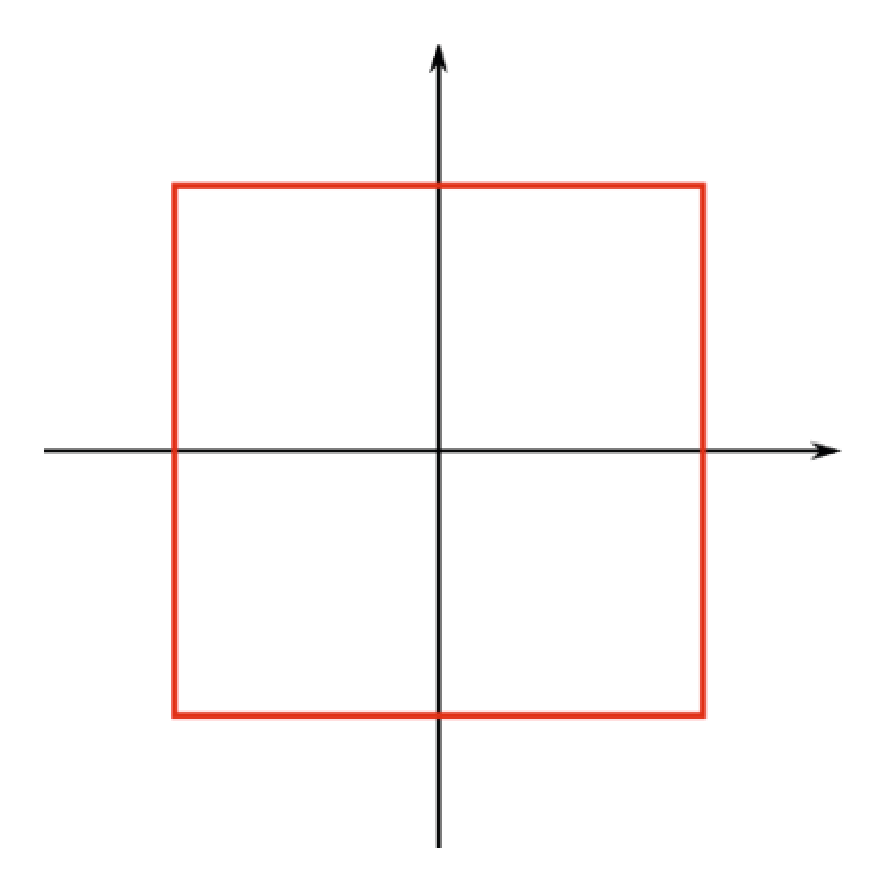
\includegraphics[scale=0.35]{fig3_1} 
		\figcaption{正方形}
	}
	
	\marginpar{
		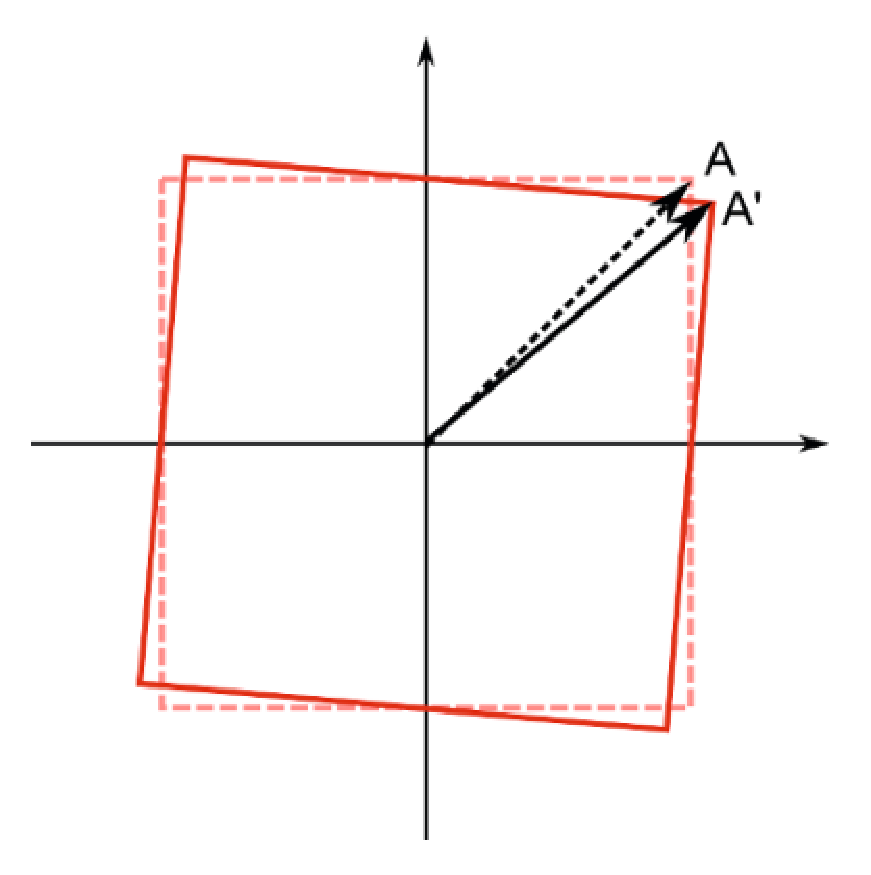
\includegraphics[scale=0.35]{fig3_2.eps}
		\figcaption{正方形绕中心顺时针旋转$5^\circ$}
	}
	
	注意不是所有旋转变换都对称。 我们关注顶点的变化就能看出来, 比如绕中心顺时针旋转$5^\circ$, 这个变换将顶点映射到原来正方形点集之外, 顶点$A$映射到了原来正方形集合之外的点$A'$。 因此这个旋转变换对正方形不具有对称性。 当然, 变换后的点集仍然是个正方形, 但却是不同的正方形(即不同点的集合)。 绕中心转$90^\circ$是对称的, 如图\ref{fig3.3}, 顶点$A$变换到点$B$, 等等, 原来的正方形点集变换到相同的集合。
	
	{
	\centering{
	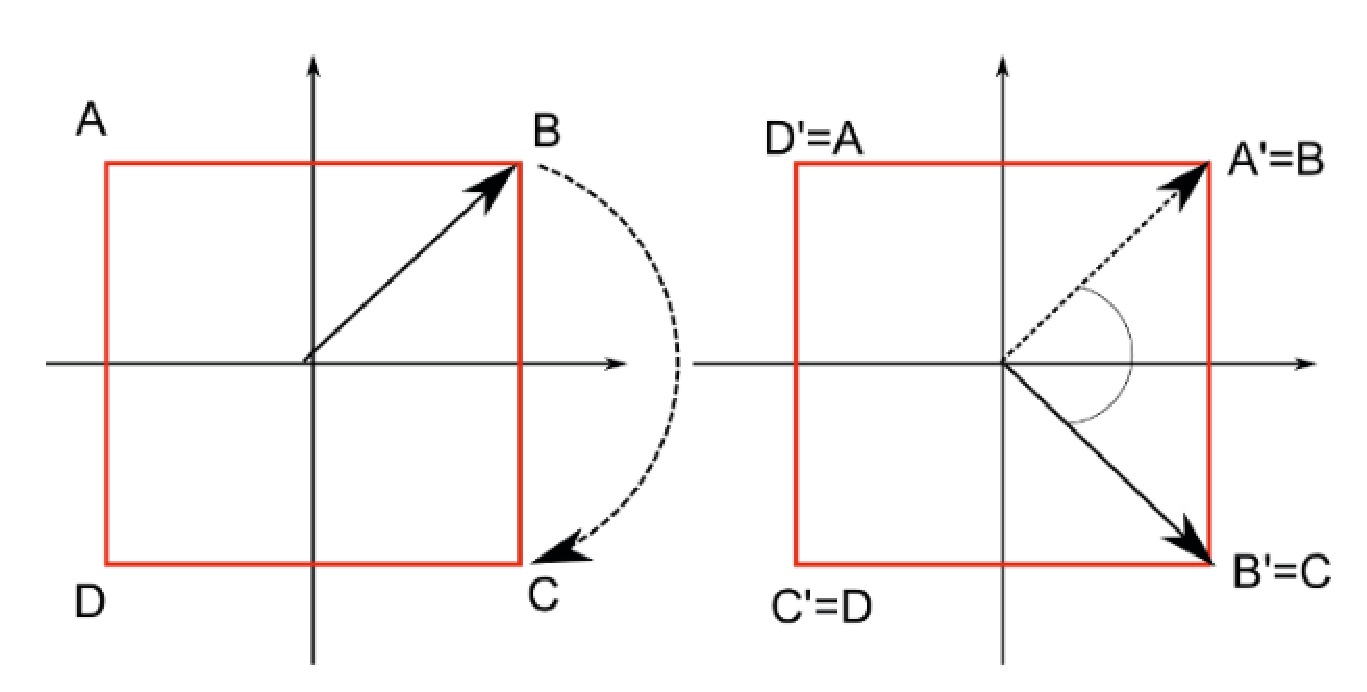
\includegraphics[scale=0.4]{fig3_3}
	\figcaption{正方形绕中心旋转$90^\circ$}
	\label{fig3.3}
	}}
	
	假如你看了一眼原来的正方形, 然后闭上眼睛, 这时有人把正方形做了一个变换。 如果你不能分辨这个正方形是否发生变化, 那么这个变换就是个对称变换。
	
	我们把所有使正方形不变的变换构成的集合称为群。 变换参数(本例中就是旋转角度)不能任意取值(而是取分立的数), 这个群称为离散群。
	
	\item 另一个例子是使单位圆不变的变换构成的集合。 类似地, 单位圆还是一些点构成的集合, 对称变换把这个集合映射到它自身。
	
	单位圆绕圆心旋转任意角度都不变。 换言之, 变换参数(这里就是旋转角度)可以取任意值, 因此这个群称为连续群。
\end{enumerate}
	\marginpar{
		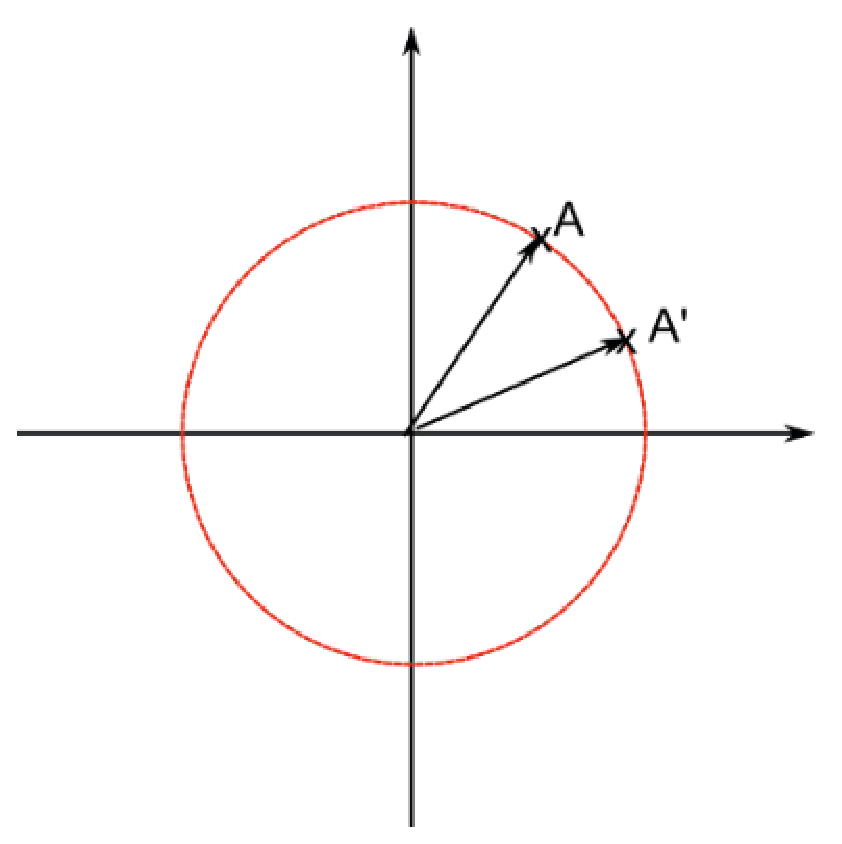
\includegraphics[scale=0.35]{fig3_4.eps}
		\figcaption{单位圆绕圆心旋转任意角度都不变}
	}

数学中除了几何图形之外还有好多别的都有对称性。 例如,对于向量, 我们可以考虑所有让向量长度不变的变换构成的集合。 看出本节开头对称性定义的普遍性了没? 对称性就是变换下的不变性。 非常幸运, 搞数学的早已建立了群论, 它可以研究所有类型的对称性\mpar{历史上数学家们建立群论最初是为了描述方程的对称性}。

为了让精确描述对称性的工具 --- 群的定义来的自然一点, 我们把对称性的定义用数学语言精炼一下:
\begin{itemize}
	\item 对某物什么也不做(比如转个$0^\circ$)当然也是对称变换(按照我们的对称性定义), 因此任何群都需要包含一个恒等变换(恒等元)。 在上面的例子里, 恒等元就是旋转$0^\circ$。
	
	\item 对某物先做变换再做逆变换的结果必须等于啥也不做。 因此对于群中的任意元素(简称群元), 必须有相应的逆元素。 按定义, 先做变换再做逆变换等于恒等变换。 例如先转$90^\circ$再转$-90^\circ$(先逆针再顺针转)与旋转$0^\circ$相同。
	
	\item 先做一个对称变换再做一个对称变换, 总体效果必须还是对称变换。 例如先旋转$90^\circ$再转$180^\circ$等于直接转$270^\circ$, 后者也是对称变换。 对称变换的这个性质称为封闭性。
	
	\item 对称变换之间必须满足结合律。 例如先转$90^\circ$再转$40^\circ$再转$110^\circ$与先转$130^\circ$再转$110^\circ$相同, 先转$90^\circ$再转$150^\circ$也一样。 用符号表示更加清楚:
	\begin{equation}\label{equ3.1}
	R(110^\circ) R(40^\circ) R(90^\circ) = R(110^\circ)\bigg( R(40^\circ)R(90^\circ) \bigg) = R(110^\circ) R(130^\circ)
	\end{equation}
	\begin{equation}\label{equ3.2}
	R(110^\circ) R(40^\circ) R(90^\circ) = \bigg( R(110^\circ) R(40^\circ) \bigg) R(90^\circ) = R(150^\circ) R(90^\circ)
	\end{equation}
	这个性质称为{\bf 结合律}。
	
	\item 我们要有规定两个群元(对称变换)怎样合体的规则, 它是个{\bf 二元运算}(两个群元合体成一个), 我们称它为{\bf 群乘法}。 
	
	在上面的例子里, 旋转变换的标准表示方法是用旋转矩阵\mpar{旋转矩阵见附录A.2.}, 两个群元(两个旋转矩阵, 或两个旋转操作)合体的规则是线性代数里的矩阵乘法。 同样的变换经常有不同的表示方法\mpar{例如, 二维平面旋转还可以用单位复数描述, 相应的群乘法是复数乘法。 稍后就讨论这一点。}, 群论非常系统性地概括了所有形式。 群论的分支 --- {\bf 表示论}就是研究相同变换的不同描述方式的, 我们在\ref{sec3.5}节学习表示论。
\end{itemize}

\ 

我们把上述群与对称变换的特征用严谨的数学语言表达, 再将它们提升为公理, 满足这些公理的数学结构就是一个群。 数学系的群论书可能更喜欢在开头就从天上掉下来这些公理。 必须指出满足群公理的结构可能是超级抽象的, 但我们现在只关注上面例子里的旋转变换那样的群。 \sout{因为我们是物理系的, 而且这是本物理书}

\ 

(我们通过对称变换的性质导出的)群公理\mpar{别担心怎么才能根据这些公理凑出一个群来。 搞物理的往往是从某个变换出发, 考察它是否符合群公理, 如果是\sout{经常是}那么就可以应用群论来解决问题。}: 

一个群就是一个集合$G$加上一个定义在$G$上的二元运算(群乘法)$\circ$, 当然$(G, \circ)$还要满足以下公理: 
\begin{itemize}
	\item 封闭性: 对于任意$g_1, g_2 \in G, g_1 \circ g_2 \in G$
	
	\item 单位元: 存在单位元$e \in G$使得对于所有$g \in G, g\circ e = g = e \circ g$
	
	\item 逆元: 对于任意$g \in G$, 存在相应的逆元$g^{-1} \in G$使得$g \circ g^{-1} = e = g^{-1} \circ g$
	
	\item 结合律: 对于任意$g_1, g_2, g_3 \in G, g_1 \circ (g_2 \circ g_3) = (g_1 \circ g_2) \circ g_3$ 
\end{itemize}

总结: 某物体在一些变换下保持不变, 这些变换组成\footnote{我在想这里该用`构成'还是`组成', 后来我觉得无所谓, 因为这不是初中化学...(分子构成物质, 元素组成物质...) --- 译者(SI)}的集合叫做对称群。 对于Minkowski时空, Minkowski度规\mpar{复习一下, Minkowski度规就是在Minkowski空间中用来计算距离和长度的工具, 见第二章。}在变换下保持不变, 相应的对称群称为Poincare群。

要注意群的定义完全与变换的物体是啥没有关系。 我们可以脱离特定物体而只研究对称变换本身, 群的定义将变换从物体中`提取'出来了。 这是非常有用的, 许多不同事物具有同样或同类的对称性。 群论让我们不用管变换的物体(圆还是正方形), 只研究变换(例如旋转)的普遍性质。


\section[二维旋转]{Rotations in two Dimensions\quad 二维旋转}
\label{sec3.2}
我们从一个简单而重要的例子开始学习群论。考虑那些让二维平面中的向量长度不变的对称变换。符合条件的有旋转和反射\mpar{当然还有平移。平移的数学描述与前两者有些不同,我们之后再讨论它。}。它们也是圆的对称变换,一个单位元旋转或反射之后还是单位圆。可见同一个群(对应一种变换)可以作用于不同类物体:圆(几何图形),或者向量。本节考虑向量,可以用旋转矩阵表示向量的旋转或反射,\mpar{旋转矩阵的推导见附录A.2.},将起点位于原点的向量绕原点逆时针旋转$\theta$角度的旋转矩阵为:
\begin{equation}
\label{equ3.3}
R_\theta = 
	\begin{pmatrix}
		\cos \theta & \sin \theta \\
		-\sin \theta & \cos \theta
	\end{pmatrix}
\end{equation}

关于$x$轴与$y$轴的反射变换用矩阵表示为:
\begin{equation}
\label{equ3.4}
P_x = 	\begin{pmatrix}
			-1 & 0 \\ 0 & 1
		\end{pmatrix}
\quad
P_y = 	\begin{pmatrix}
			1 & 0 \\ 0 & -1
		\end{pmatrix}
\end{equation}
将矩阵乘法作为群乘法$\circ$, 可以验证$R(\theta), P_x, P_y$与矩阵乘法符合群公理,因而构成一个群,亦即旋转与反射变换构成一个群。

可以用更抽象的方式表达‘所有让二维向量长度不变的变换’,向量长度就是向量与自身点乘的平方根($|a| = \sqrt{a \cdot a}$). 向量长度在变换$a \rightarrow a'$下不变意味着\footnote{等号上面的!只是起强调、提示作用 --- 译者(SI)}:
\begin{equation}
\label{equ3.5}
a' \cdot a' \stackrel{!}{=} a \cdot a
\end{equation}

将变换矩阵记作$\mathcal{O}$,变换即为$a \rightarrow a' = \mathcal{O}a$.
\begin{equation}
\label{equ3.6}
a \cdot a = a^{\mathrm{T}} a \rightarrow a'^{\mathrm{T}} a' = (\mathcal{O} a)^{\mathrm{T}} \mathcal{O} a = a^{\mathrm{T}} \mathcal{O}^{\mathrm{T}} \mathcal{O} a \stackrel{!}{=} a^{\mathrm{T}} a = a \cdot a
\end{equation}
由此可见,使向量长度不变的变换必须满足:
\begin{equation}
\label{equ3.7}
\mathcal{O}^{\mathrm{T}} \mathcal{O} = I
\end{equation}
其中$I$表示单位矩阵\mpar{ I = 
	\[\begin{pmatrix}
		1 & 0 \\ 0 & 1
	\end{pmatrix}\]}。前文的旋转和反射矩阵都满足此条件\mpar{例如\ref{equ3.3}式的矩阵,
	$R_\theta^{\mathrm{T}} R = 
	\begin{pmatrix}
		\cos \theta & -\sin \theta \\
		\sin \theta & \cos \theta
	\end{pmatrix}
	\begin{pmatrix}
		\cos \theta & \sin \theta \\
		-\sin \theta & \cos \theta
	\end{pmatrix}
	 = 
	 \begin{pmatrix}
		 \cos^2 \theta + \sin^2 \theta & 0 \\
		 0 & \sin^2 \theta + \cos^2 \theta
	 \end{pmatrix}
	 =
	 \begin{pmatrix}
		 1 & 0 \\ 0 & 1
	 \end{pmatrix}
	$
}%mpar
$2 \times 2$矩阵中所有满足\ref{equ3.7}式的矩阵构成了$\mathcal{O}(2)$群,即所有$2 \times 2$正交矩阵构成的群\mpar{严谨地说,任意$2 \times 2$正交矩阵可以表示为\ref{equ3.3}、\ref{equ3.4}式,或者它们的乘积的形式。}。我们可以找出这个群中描述旋转变换的那一部分(构成一个子群)。根据\ref{equ3.7}式:
\begin{align}
\det(\mathcal{O}^{\mathrm{T}} O ) = \det(O^{\mathrm{T}}) \det(O) \stackrel{!}{=} \det(I) = 1 \nonumber\\
\label{equ3.8}
(\det(\mathcal{O}))^2 \stackrel{!}{=} 1 \rightarrow \det{(\mathcal{O})} \stackrel{!}{=} \pm 1
\end{align}

$\det \mathcal{O} = 1$的矩阵对应旋转变换\mpar{见\ref{equ3.3}与\ref{equ3.4}式。反射矩阵的行列式等于$-1$。}

条件
\begin{align}
\label{equ3.9}
\mathcal{O}^{\mathrm{T}} \mathcal{O} = I \\
\label{equ3.10}
\det \mathcal{O} = 1
\end{align}
定义了$\mathcal{SO}(2)$群,`$\mathcal{S}$'表示‘特殊’(special),`$\mathcal{O}$'表示‘正交’(orthogonal)。

$\mathcal{SO}(2)$包含的旋转变换保持了坐标系的取向,即一个右手坐标系\mpar{右手坐标系与左手坐标系见附录A.5.}经旋转变换后还是右手系,而反射变换会改变它的取向。用线性代数的概念来说,我们规定$\mathcal{SO}(2)$中的矩阵行列式必须为$+1$。

\subsection[单位复数表示旋转变换]{Rotations with Unit Complex Numbers\quad 单位复数表示旋转变换}
\label{sec3.2.1}
还可以用单位复数来表示旋转变换:向量绕原点旋转$\theta$角可以表示为用单位复数$z$乘此向量(单位复数意为$z = a + ib$,$|z|^2 = z^* z = 1$)\mpar{上标$ ^*$表示复数的共轭复数:$z = a + ib \rightarrow z^* = a - ib$}。

所有单位复数构成一个群,称为$\mathcal{U}(1)$,群乘法即为复数乘法,不难验证它符合群公理。为了看出它与之前引入的$\mathcal{O}(3), \mathcal{SO}(3)$群的关系,我们将$\mathcal{U}(1)$群的条件 --- 单位复数表示为\mpar{定义中包含复数乘法的群的普遍性质见\ref{sec3.10}节的附录。}, $\forall \mathcal{U} \in \mathcal{U}(1)$:
\begin{equation}
\label{equ3.11}
\mathcal{U}^* \mathcal{U} = 1
\end{equation}
单位复数另一种形式是利用欧拉公式\mpar{附录B.4.2推导了传说中的欧拉公式。对任意复数$z = a + ib$, $a$称为$z$的实部,记为$\Re(z) = a$; $b$称为虚部,记为$\Im(z) = b$. 欧拉公式中$R_\theta$的实部为$\cos  \theta$, 虚部为$\sin \theta$.}:% Euler翻译为欧拉
\begin{equation}
\label{equ3.12}
R_\theta = \mathrm{e}^{i\,\theta} = \cos \theta + i\sin \theta
\end{equation}
$R(\theta)$的模(长度)为:
\begin{equation}
\label{equ3.13}
R_\theta^* R_\theta = \mathrm{e}^{-i\,\theta} \mathrm{e}^{i\,\theta} = \big( \cos \theta - i \sin \theta  \big) \big( \cos \theta + i \sin \theta \big) = 1
\end{equation}

\marginpar{
	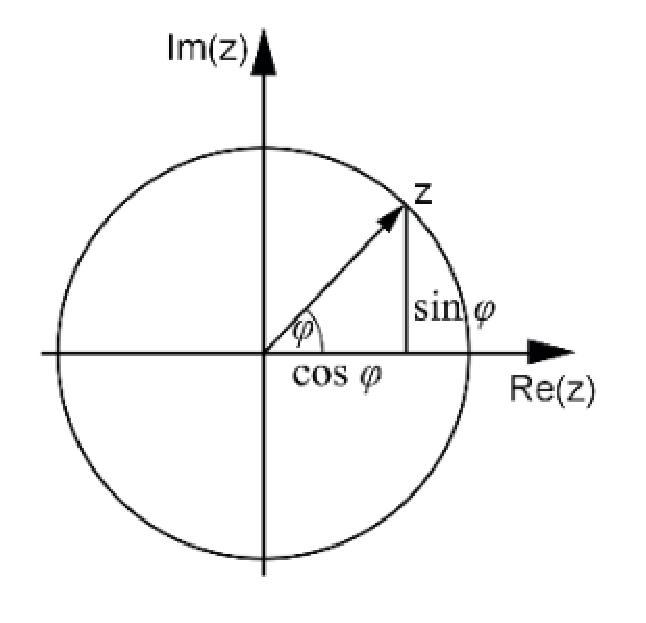
\includegraphics[scale=0.45]{fig3_5.eps} 
	\figcaption{单位复数在复平面的单位圆上}
	}

例:将向量$(3,  5)$旋转$90^\circ$:
\begin{equation}
\label{equ3.14}
z \rightarrow z' = \mathrm{e}^{i\, 90^\circ}z = \bigg( \underbrace{\cos 90^\circ}_{=0} + i\underbrace{\sin 90^\circ}_{=1} \bigg) (3 + 5i) = i(3 + 5i) = 3i - 5
\end{equation}

图3.6绘制了旋转前后的向量(复数),图中可见复数乘以$\mathrm{e}^{i\, 90^\circ}$旋转了$90^\circ$.
\marginpar{
	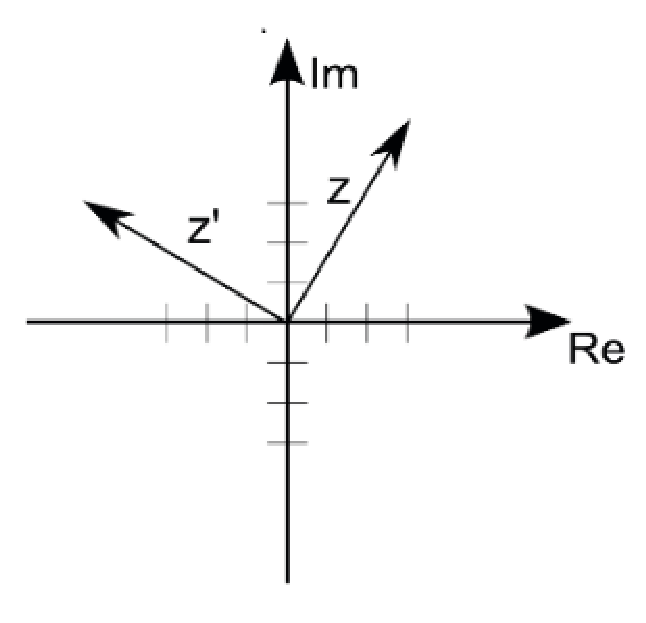
\includegraphics[scale=0.45]{fig3_6.eps} 
	\figcaption{复数通过乘以单位复数进行旋转}
	}
需要注意$\mathrm{e}^{i\, 90^\circ}$作用于(乘以)向量对应的复数而非向量本身。描述二维旋转只需要一个参数:旋转角$\phi$. 而复数有两个自由度(实部和虚部),因此我们加上单位复数的限制:$|z| = \text{实部}^2 + \text{虚部}^2 = 1$,只剩一个自由度。

描述二维旋转的两种方式 --- 单位复数与$2 \times 2$矩阵(矩阵元都是实数)通过如下方式关联。定义:
\begin{equation}
\label{equ3.15}
\mathbf{1} = 
	\begin{pmatrix}
		1 & 0 \\ 0 & 1
	\end{pmatrix}
,\quad
\mathbf{i} = 
	\begin{pmatrix}
		0 & -1 \\ 1 & 0
	\end{pmatrix}
\end{equation}
不难验证这样定义的$\mathbf{1, i}$仍然满足:
\begin{equation}
\mathbf{1}^2 = \mathbf{1},\quad \mathbf{i}^2 = -\mathbf{1},\quad \mathbf{1i} = \mathbf{i1} = \mathbf{i}
\end{equation}
这样单位复数对应的$2 \times 2$实数矩阵为\footnote{原文此式有误,译文已参照勘误表修改。}
\begin{equation}
\label{equ3.17}
R_\theta = \cos \theta + i\sin\theta = \cos \theta 
\begin{pmatrix}
	1 & 0 \\ 0 & 1
\end{pmatrix}
+ \sin \theta
\begin{pmatrix}
	0 & -1 \\ 1 & 0
\end{pmatrix}
=
\begin{pmatrix}
	\cos \theta & -\sin \theta \\
	\sin \theta & \cos \theta
\end{pmatrix}
\end{equation}
可见,定义了复单位$i \rightarrow \text{实矩阵}$的对应关系后,单位复数就回到了熟悉的旋转矩阵。还有一点要注意:旋转矩阵作用于向量(列矩阵),而我们将$i$与$2 \times 2$矩阵相联系,因此被旋转的向量(与一个复数对应)也将变成一个$2 \times 2$矩阵。

例:任意向量$(a, b)$对应的复数对应的$2 \times 2$矩阵为:
\begin{equation}
\label{equ3.18}
z = a + ib = a
\begin{pmatrix}
	1 & 0 \\ 0 & 1
\end{pmatrix}
+ b
\begin{pmatrix}
	0 & -1 \\ 1 & 0
\end{pmatrix}
=
\begin{pmatrix}
	a & -b \\ b & a
\end{pmatrix}
\end{equation}
将旋转矩阵作用于$z$:
\begin{eqnarray}
\label{sec3.19}
	z' &=& \begin{pmatrix}
			a' & -b' \\ b' & a'
		 \end{pmatrix}
	= R_\theta z = 
		\begin{pmatrix}
			\cos \theta & -\sin \theta \\
			\sin \theta & \cos \theta
		\end{pmatrix}
		\begin{pmatrix}
			a & -b \\ b & a
		\end{pmatrix}
	\nonumber \\
	&=& \begin{pmatrix}
			a\cos\theta - b\sin \theta & - b\cos \theta - a \sin \theta \\
			a\sin \theta + b\cos \theta & -b \sin \theta + a \cos \theta
		\end{pmatrix}
\end{eqnarray}
由上式可得
\begin{align}
\label{equ3.20}
a' &= a \cos \theta - b \sin \theta \\
\label{equ3.21}
b' &= a \sin \theta + b \cos \theta
\end{align}
这与旋转矩阵作用于向量(列矩阵形式)相同:
\begin{equation}
\label{equ3.22}
	\begin{pmatrix}
		\cos \theta & -\sin \theta \\
		\sin \theta & \cos \theta
	\end{pmatrix}
	\begin{pmatrix}
		a \\ b
	\end{pmatrix}
	=
	\begin{pmatrix}
		a \cos \theta - b \sin \theta \\
		a \sin \theta + b \cos \theta
	\end{pmatrix}
	=
	\begin{pmatrix}
		a' \\ b'
	\end{pmatrix}
\end{equation}
我们看到这两种表示方法是一回事儿,用数学术语来说,$\mathcal{SO}(2)$与$\mathcal{U}(1)$间有一个同构映射\mpar{如果映射$\Pi: G \rightarrow G'$是一一映射,并且满足:$\forall g_1, g_2 \in G, \Pi(g_1) \circ \Pi(g_2) = \Pi(g_1 \circ g_2)$, 则$\Pi$就是同构映射,并且称群$G, G'$是同构的。}。这一点太重要了,之后的篇幅会不断出现这种思想。

下面研究三维旋转,尝试找出它的两种描述方法。

\section[三维旋转]{Rotations in three Dimensions\quad 三维旋转}
\label{sec3.3}
三维空间向量旋转变换当然可以用$3 \times 3$旋转矩阵\footnote{原文公式有误,译文已按勘误表改正。}:
\begin{align}
R_x =
	\begin{pmatrix}
		1 & 0 & 0 \\
		0 & \cos \theta & -\sin \theta \\
		0 & \sin \theta & \cos \theta
	\end{pmatrix}
\quad
R_y = 
	\begin{pmatrix}
		\cos \theta & 0 & \sin \theta \\
		0 & 1 & 0 \\
		-\sin \theta & 0 & \cos \theta
	\end{pmatrix}
\nonumber \\
\label{equ3.23}
R_z =
	\begin{pmatrix}
		\cos \theta & -\sin \theta & 0 \\
		\sin \theta & \cos \theta & 0 \\
		0 & 0 & 1
	\end{pmatrix}
\end{align}
类比$\mathcal{SO}(2)$群,上面三个矩阵构成了$\mathcal{SO}(3)$群的一组基\mpar{基的概念见附录A.1.}。这意味着$\mathcal{SO}(3)$中的任意群元(矩阵)都可以写为$R_x, R_y, R_z$的线性组合,且系数唯一。
将向量
\begin{equation*}
\vec{v} = \begin{pmatrix}
			1 \\ 0 \\ 0
		\end{pmatrix}
\end{equation*}
绕$z$轴旋转\mpar{三维向量旋转的一般情况的推导见附录A.2.}就是用旋转矩阵乘以向量:
\begin{equation}
\label{equ3.24}
R_z(\theta) \vec{v} = 
	\begin{pmatrix}
		\cos \theta & -\sin \theta & 0 \\
		\sin \theta & \cos \theta & 0 \\
		0 & 0 & 1
	\end{pmatrix}
	\begin{pmatrix}
		1 \\ 0 \\ 0
	\end{pmatrix}
=
	\begin{pmatrix}
		\cos \theta \\ \sin \theta \\ 0
	\end{pmatrix}
\end{equation}
为找出描述三维旋转的第二法,我们尝试把复数的概念扩展到三维空间。首先试着把$2$维的复数(实部虚部两个自由度)扩展为$3$维复数,但前人探索发现没有$3$维的,但存在$4$维‘复数’,称为{\bf 四元数(quaternions)}。下面就会看到四元数正是描述三维旋转的第二法,并且它还能深刻揭示宇宙 --- 四维时空的规律。描述三维旋转需要三个参数(绕$x,y,z$轴的旋转角),而四元数有四个参数,这与二维旋转的情况类似\mpar{单位复数描述二维旋转。}。四元数加上单位长度的限制 ---单位四元数(三个自由参数)能够描述三维旋转。

\subsection[四元数]{Quaternions\quad 四元数}
